\capitulo{6}{Trabajos relacionados}

En este apartado se recogen todas las aplicaciones y proyectos que ofrecen funcionalidades parecidas a las que se implementan en eLearningQA. Como en un estudio de mercado se comprueba que ofrecen otras personas o entidades para identificar las necesidades que se pueden cubrir. 

\section{Moodle Course Checker}
Course Checker \cite{moodle-course-checker} es un plugin de Moodle que ofrece la posibilidad de hacer hasta diez comprobaciones comparativas entre cursos propias de la fase de implementación. Este plugin permite corregir fallos en la configuración de cursos con el fin de mantener una consistencia interna entre los distintos cursos.

\section{Course Check Blocks}
Course Check Blocks \cite{course-checks-blocks} es un plugin que ofrece 11 comprobaciones automáticas que permiten al usuario mantener un mínimo de calidad en el curso y aumentar las oportunidades de mejora. Además ofrece una funcionalidad adicional que permite borrar cualquier bloque vacío del curso.

\section{Dashboard for Evaluating the Quality of Open Learning Courses}
Un artículo \cite{modelo-sustanabilty} publicado en la revista Sustainbility por Gina Mejía-Madrid, Faraón Llorens-Largo, y Rafael Molina-Carmona en 2020, presenta un modelo para la evaluación de calidad en cursos, así como, un panel visual que permite ver los resultados obtenidos y compararlos de forma rápida y sencilla.

\section{A Hierarchical Model to Evaluate the Quality of Web-Based E-Learning Systems}
En un estudio publicado en la revista Sustainability por Abdul Hafeez Muhammad y otros miembros de varias universidades \cite{marco-calidad-muhammad}, muestra un modelo que determina cuales son los factores más relevantes a tener en cuenta para mantener un curso con calidad. Para la obtención de este modelo se encuestaron a 157 sujetos para obtener los criterios más importantes para la calidad de un curso, una vez obtenidos esos criterios se les proporcionó a 51 sujetos esos criterios para compararlos entre sí para obtener la importancia de cada uno de ellos.

Así pues, el modelo obtenido \ref{fig:marco-muhammad} se puede utilizar como marco para el desarrollo de cursos de calidad, es interesante tener en cuenta este trabajo por que, como otros modelos, también proporciona un marco para el diseño de cursos en línea de calidad.

\begin{figure}[H]
    \centering
    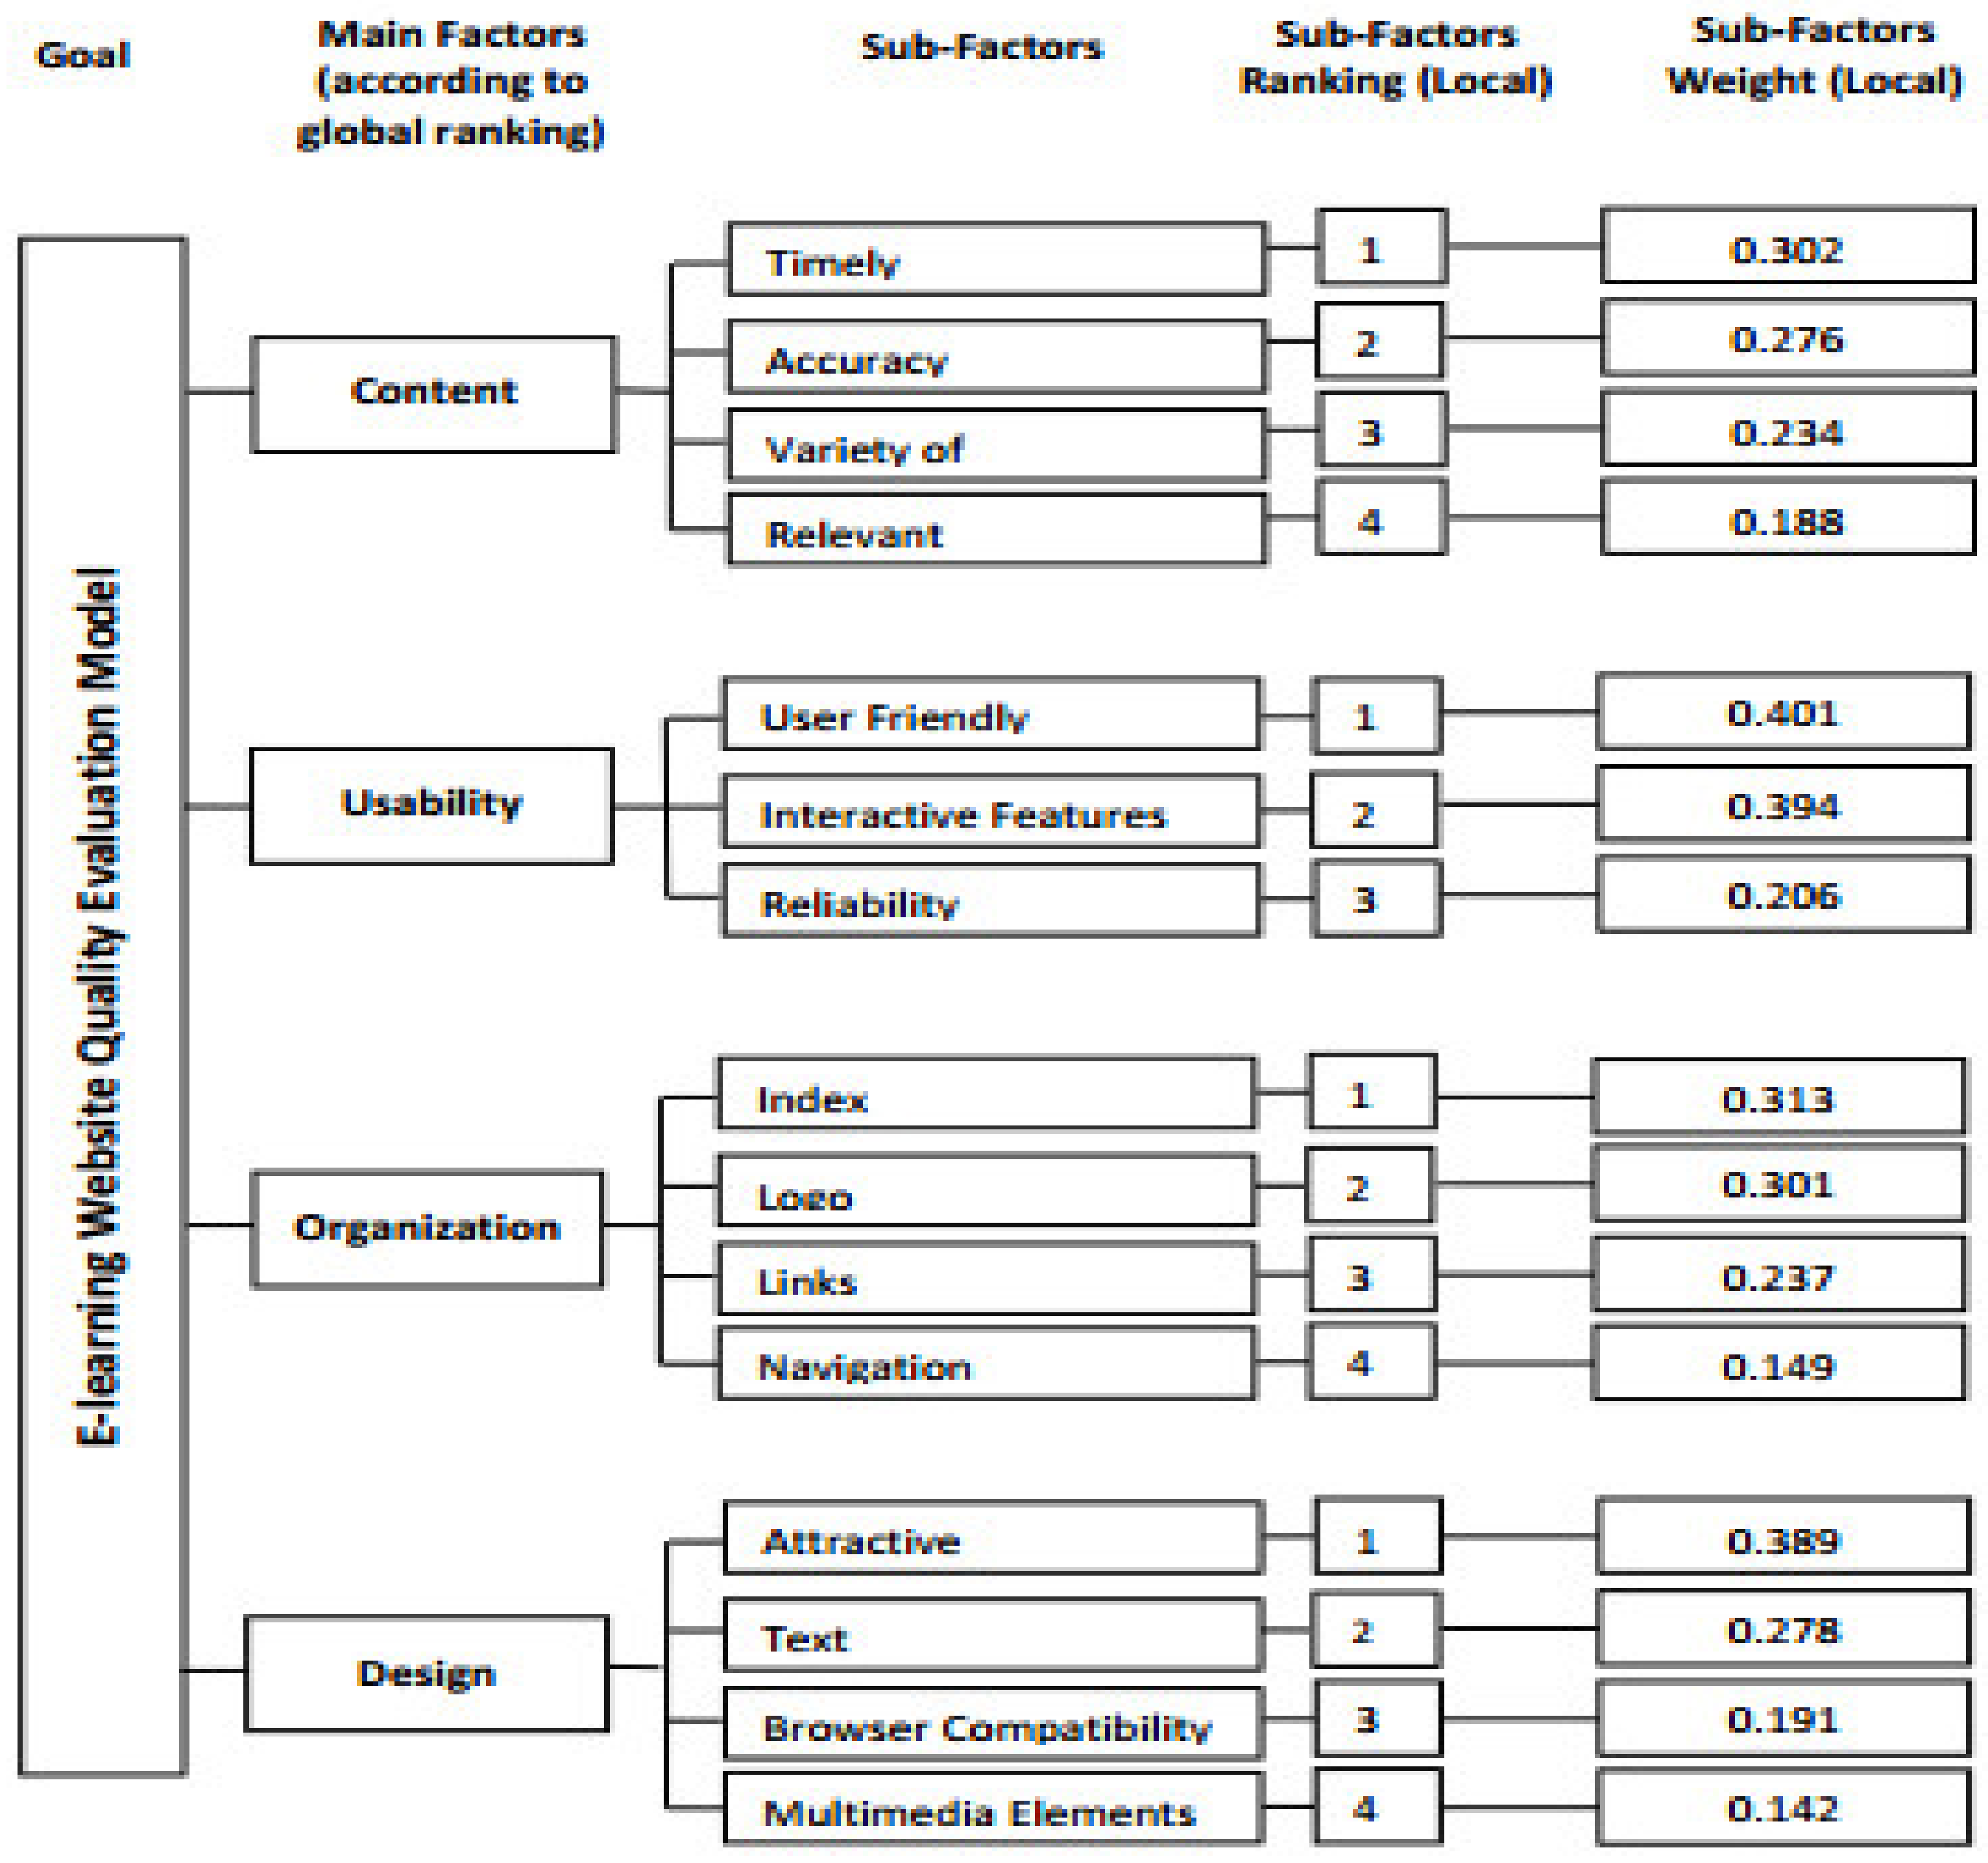
\includegraphics[width=1\linewidth]{img/modelo-evaluacion-calidad.png}
    \label{fig:marco-muhammad}
    \caption{Marco de calidad definido en ``Hierarchical Model to Evaluate the Quality of Web-based E-Learning Systems''}
\end{figure}


\section{Comparación entre trabajos relacionados y eLearningQA}
Finalmente, con todas las opciones que se han visto, se puede hacer una comparativa con eLeaarningQA.

\begin{table}[H]
\resizebox{\textwidth}{!}{%
	\begin{tabular}{l|ccc}
		\hline
		\rowcolor[HTML]{FFFFFF} 
		\textbf{Característica} & \textbf{eLearningQA} & \textbf{Course Checker} & \textbf{
            \begin{tabular}[c]{@{}c@{}}
                Course Checks\\ Block
            \end{tabular}}         
        \\ \hline
        
		\rowcolor[HTML]{EFEFEF} 
		Idiomas & Español & \begin{tabular}[c]{@{}c@{}}Español, inglés,\\ alemán, y portugués\end{tabular} & \begin{tabular}[c]{@{}c@{}}Español, inglés,\\ portugués, y griego\end{tabular} \\
		Nº de comprobaciones &23 & 10 & 8\\
		\rowcolor[HTML]{EFEFEF} 
		\begin{tabular}[c]{@{}l@{}}Ejecución independiente\\ de comprobaciones\end{tabular} & No & Sí & No\\
		\begin{tabular}[c]{@{}l@{}}Contiene enlaces para\\ solventar los problemas\end{tabular} & Sí & Sí & No\\
		\rowcolor[HTML]{EFEFEF} 
		\begin{tabular}[c]{@{}l@{}}Versiones de Moodle\\ compatibles\end{tabular}& v3.8+ & v3.6+ & v2.6+\\
		Tipo & Aplicación web & Plugin & Plugin\\ \hline
	\end{tabular}%
}
\end{table}





